\documentclass{article}

\usepackage{fancyhdr}
\usepackage{extramarks}
\usepackage{amsmath}
\usepackage{amsthm}
\usepackage{amsfonts}
\usepackage{tikz}
\usepackage[plain]{algorithm}
\usepackage{algpseudocode}
\usepackage{textcomp}
\usepackage{graphicx}
\usepackage{subcaption}

\usepackage{tikz-timing}
\usetikztiminglibrary[rising arrows]{clockarrows}

\usetikzlibrary{automata,positioning}
\usepackage[shortlabels]{enumitem}
%
% Basic Document Settings
%

\topmargin=-0.45in
\evensidemargin=0in
\oddsidemargin=0in
\textwidth=6.5in
\textheight=9.0in
\headsep=0.25in

\linespread{1.1}

\renewcommand\headrulewidth{0.4pt}
\renewcommand\footrulewidth{0.4pt}

\setlength\parindent{0pt}

\begin{document}

\section{Motivation for Taking Discrete Fourier Transforms}

The Discrete Fourier is used to transform a finite length $N$ sequence of samples in the time domain to its eneries
in $N$ discrete frequencies. This is useful both for spectrum analysis, but also for filtering. As in certain cases
(where you can avoid cirular effects), convolution in the time domain maps to multiplication in the frequency domain.
This means we could take the transform of both our signal and our filter, multiply them, and take the inverse transform,
rather than implementing a filter directly (which may be quite costly).

\section{FFT Theory}
The FFT (Fourier Transform) is is algorithm to compute the DFT (Discrete Fourier Transform) with less hardware, taking advantage
of some symetries of the transform that work specifically when the $N$ is a power of 2.

Define $W_{N}$

\begin{equation*} W_{N} = e^{-j \frac{2 \pi}{N}} \end{equation*}

Note these symetries:

\begin{align*}
  W_{N}^{k+N/2} &= W_{N}^{k}W_{N}^{N/2} &= -W_{N}^{k} \\
  W_{N}^{k+N}   &= W_{N}^{k}W_{N}^{N}   &= W_{N}^{k} \\
\end{align*}

Then the DFT can be experessed as:

\begin{equation}  X_{N}[k] = \sum_{n=0}^{N-1} x[n] W_{N}^{kn} \end{equation}

Notice that this requires N multiplications and N summations for each $X[k]$, for a total of $N^{2}$ multiplies.

There are two main ways to divide the DFT into similar bits of computation,
\emph{Decimation in Frequency} and \emph{Decimation in Time}.

Define N-bitreverse order as reversing the binary representation of a number, ie

\begin{tabular}{ | r | r | r | r | }
    \hline
    Natural Order (Dec) & Natural Order(Bin) & Bit Reverse(Bin) & Bit Reverse (Dec) \\
    \hline
    0 & 3b000 & 3b000 & 0 \\
    1 & 3b001 & 3b100 & 4 \\
    2 & 3b010 & 3b010 & 2 \\
    3 & 3b011 & 3b110 & 6 \\
    4 & 3b100 & 3b001 & 1 \\
    5 & 3b101 & 3b101 & 5 \\
    6 & 3b110 & 3b011 & 3 \\
    7 & 3b111 & 3b111 & 7 \\
    \hline
\end{tabular}

Bit reverse order will come up as we compute FFTs.

In general, if the input is in Natural Order, \emph{Decimation in Frequency} is more natural, while if the input is in
Bit reverse order, \emph{Decimation in Time} is more natural.

\pagebreak
\subsection{Decimation in Frequency}

\begin{align*}
    X_{N}[k] &= \sum_{n=0}^{N/2-1} x[n] W_{N}^{kn} + &                     & \sum_{n=N/2}^{N-1} x[n] W_{N}^{k} \\
    X_{N}[k] &= \sum_{n=0}^{N/2-1} x[n] W_{N}^{kn} + &                     & \sum_{n=0}^{N/2-1} x[n+\frac{N}{2}] W_{N}^{k\left(n + \frac{N}{2}\right)} \\
    X_{N}[k] &= \sum_{n=0}^{N/2-1} x[n] W_{N}^{kn} + & W_{2}^{k}           & \sum_{n=0}^{N/2-1} x[n+\frac{N}{2}] W_{N}^{n} \\
    X_{N}[k] &= \sum_{n=0}^{N/2-1} x[n] W_{N}^{kn} + & \left(-1\right)^{k} & \sum_{n=0}^{N/2-1} x[n+\frac{N}{2}] W_{N}^{n} \\
\end{align*}

let $a[n] = x[n] + x[n+\frac{N}{2}]$, $b[n] = x[n] - x[n+\frac{N}{2}]$.

\begin{minipage}{0.5\textwidth}
  \begin{align*}
    X_{N}[2m]   &= \sum_{n=0}^{N/2-1} a[n] W_{N}^{2mn} \\
    X_{N}[2m]   &= \sum_{n=0}^{N/2-1} a[n] W_{N/2}^{mn} \\
  \end{align*}
\end{minipage}
\begin{minipage}{0.5\textwidth}
  \begin{align*}
    X_{N}[2m+1] &= \sum_{n=0}^{N/2-1} b[n] W_{N}^{\left(2m+1\right)n} \\
    X_{N}[2m+1] &= \sum_{n=0}^{N/2-1} \left(b[n] W_{N}^{n} \right) W_{N/2}^{mn} \\
  \end{align*}
\end{minipage}

You can now see that the N-point DFT $X_{N}[k]$ has been reduced the combination of the N/2-point DFT of $a[n]$ and
the N/2 point FFT of $b[n]W_{N}^{n}$. This can be done recursively to simplify the computations greatly.
The $W_{N}^{n}$ terms are called the \emph{twiddle factors}.

\begin{figure}[h!]
  \begin{minipage}{0.5\textwidth}
    \centering
    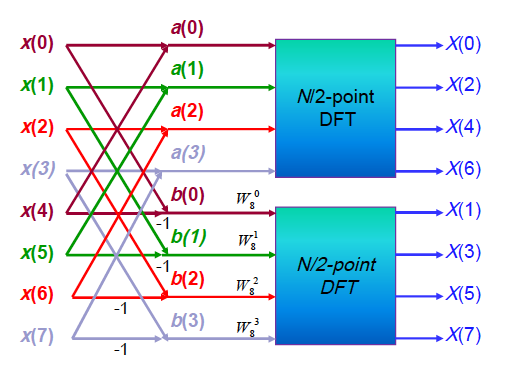
\includegraphics[width=\linewidth]{dif_1.png}
      \label{fig:dif1}
  \end{minipage}
  \begin{minipage}{0.5\textwidth}
    \centering
    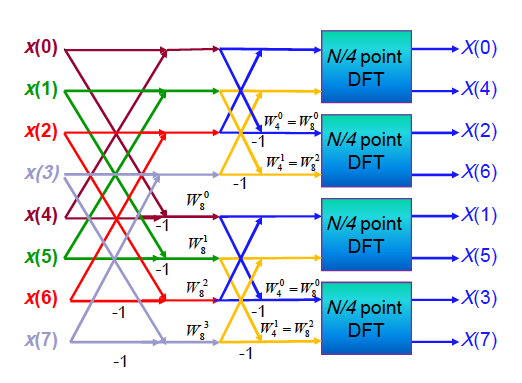
\includegraphics[width=\linewidth]{dif_2.png}
      \label{fig:dif2}
 \end{minipage}
\end {figure}

See how we could have $log2\left(N\right)$ butterfly stages, and do $2^{\emph{stage}}$ times combining of inputs from $n$ in $\left[0, 2^{\text{stage}}\right)$
\emph{left}: $a_{{stage}-1}[n]$
and \emph{right}: $b_{{stage}-1}[n]$
(using a FIFO to order the incoming data), apply twiddle factors as appropriate and output
\emph{left}: $a_{\text{stage}}[n] = a_{{stage}-1}[n] + b_{{stage}-1}[n] $
and \emph{right}: $b_{\text{stage}}[n] = a_{{stage}-1}[n] - b_{\text{stage}-1} W_{N/2^{\text{stage}}}^{n}$
It will need to keep a counter of when we are to apply each twiddle (and the last two stages with have trivial twiddles).
Also note the the input is in natural order but the output is in bitreverse order.

\pagebreak

\subsection{Decimation in Time}
\begin{align*}
    X_{N}[k] &= \sum_{n=0}^{N/2-1}x[2n] W_{N}^{2mk} + &           &\sum_{n=0}^{N/2-1}x[2n+1] W_{N}^{\left(2m+1\right)k} \\
    X_{N}[k] &= \sum_{n=0}^{N/2-1}x[2n] W_{N}^{2mk} + &           &\sum_{n=0}^{N/2-1}x[2n+1] W_{N}^{k} W_{N}^{2mk} \\
    X_{N}[k] &= \sum_{n=0}^{N/2-1}x[2n] W_{N}^{mk}  + & W_{N}^{k} &\sum_{n=0}^{N/2-1}x[2n+1] W_{N/2}^{mk} \\
\end{align*}

Let $G[k]$ be the N/2-point DFT of the even samples of $x[n]$ and let $H[k]$ be th2 N/2-point DFT of the odd samples of $x[n]$.
Note that $G[k+\frac{N}{2}] = G[k]$.


\begin{minipage}{0.5\textwidth}
  \begin{align*}
    X_{N}[k]               &= G[k]             + & W_{N}^{k}     & H[k] \\
  \end{align*}
\end{minipage}
\begin{minipage}{0.5\textwidth}
  \begin{align*}
    X_{N}[k+\frac{N}{2}]   &= G[k+\frac{N}{2}] + & W_{N}^{k+N/2} & H[k+\frac{N}{2}] \\
    X_{N}[k+\frac{N}{2}]   &= G[k+\frac{N}{2}] - & W_{N}^{k}     & H[k+\frac{N}{2}] \\
    X_{N}[k+\frac{N}{2}]   &= G[k]             - & W_{N}^{k}     & H[k] \\
  \end{align*}
\end{minipage}

You can now see that the N-point DFT $X_{N}[k]$ has been reduced to the combination of two N/2 point DFTs, $H[k]$ and $G[k]$.
This can be done recursively to simplify computations greatly. The $W_{N}^{k}$ terms are called twiddle factors.

\begin{figure}[h!]
  \begin{minipage}{0.5\textwidth}
    \centering
    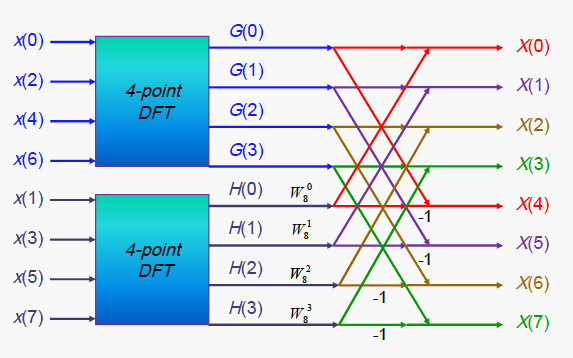
\includegraphics[width=\linewidth]{dit_1.png}
      \label{fig:dit1}
  \end{minipage}
  \begin{minipage}{0.5\textwidth}
    \centering
    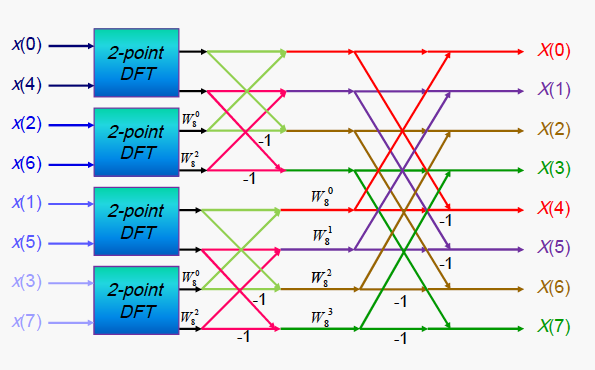
\includegraphics[width=\linewidth]{dit_2.png}
      \label{fig:dit2}
 \end{minipage}
\end {figure}

See how we could have $log2\left(N\right)$ butterfly stages, and do $N/2^{stage+1}$ combining of inputs from $k$ in $\left[0, 2^{\text{stage}}\right)$
(using a FIFO to order the incoming data), apply twiddle factors as appropriate and output
\emph{left}: $G_{\text{stage}}[k]=G_{\text{stage}-1}[k]+W_{N/2^{\text{stage}}}^{k} H_{\text{stage}-1}[k]$
and \emph{right}: $H_{\text{stage}}[k]=G_{\text{stage}-1}[k]-W_{N/2^{\text{stage}}}^{k} H_{\text{stage}-1}[k]$
It will need to keep a counter of where we are to apply each twiddle (and the first two stages with have trivial twiddles).
Also note the the input is in bitreverse order but the output is in natural order.

\pagebreak

\subsection {IFFT}
The equation for the Inverse FFT is quite similar to that of the the FFT, except that there is a factor of N that needs to be dealt with,
and the twiddle factor at each stage is the complex conjugate of its value in the corresponding FFT stages.
Therefore, we can implement it the same way as we implemented the FFT (just adjusting the ROM values appropriately).

      \begin{equation} x[n] = \frac{1}{N} \sum_{k=0}^{N-1}X[k] W_{N}^{kn} \end{equation}

The IFFT can be implemented using either the \emph{Decimation in Time} or the \emph{Decimation in Frequency} approach.

\pagebreak
\section{FFT Implementation}

Below is shown an efficient, pipelined, hardware implementation of the 8-point FFT using \emph{Decimation in Time}
and an associated timing diagram.
We use buffers because each stage of the FFT will have a distance of N/2 between input samples to put into the butterfly unit.
The same principles can be applied to compute any $2^{M}$ point FFT.

Note that the result comes out in "bitreverse" order can use a ram buffer at the end to correct this.
The butterfly units will need to have Roms with Twiddle factors and keep an internal state to know when to apply each one. \\
Notice that there is one only Butterfly unit perstage, so only one complex multiply per stage, meaning we only use about 4*log(N) real multipliers. \\
Each Stage \emph{m} will need $N/(2^{\text{m+1}})$ storage for each its input buffer and output buffer for data alignment. \\
Note that each butterfly is only active for half the time.

  \begin{figure}[h!]
    \centering
    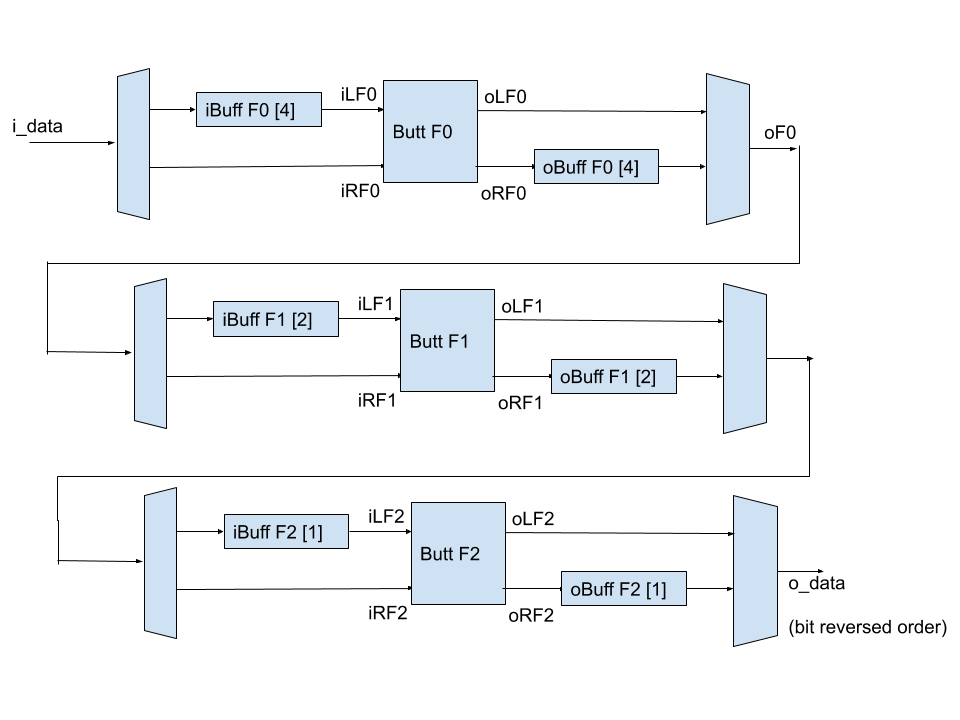
\includegraphics[width=0.8\linewidth]{pipelined_fft.png}
    \label{fig:fft}
    \caption{8-point Decimation in Time Pipelined FFT}
  \end {figure}

\pagebreak

\section{Implementing FIR Filters with FFTs Using Overlap Add}

  \begin{figure}[h!]
    \centering
    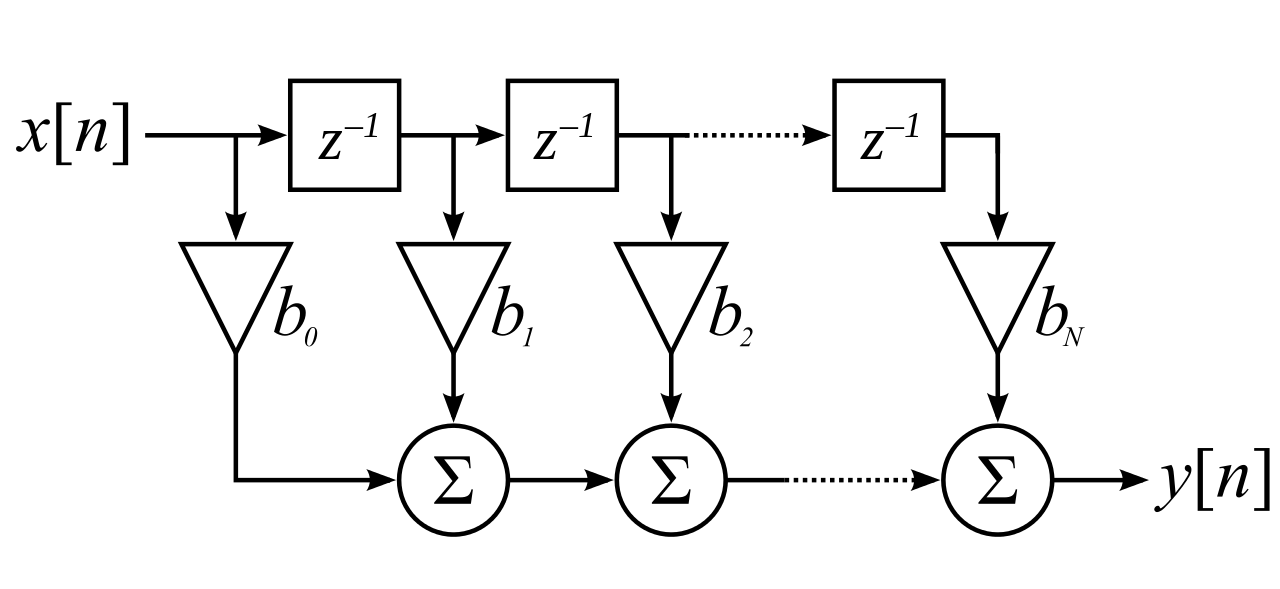
\includegraphics[width=0.6\linewidth]{firfilter.png}
    \label{fig:timedomain_fir}
    \caption{Time domain FIR Filtering}
  \end {figure}

One of the main advantages of taking Fourier Transforms is that convolution in the time domain is equivalent to multiplication
in the frequency domain. That means that we can take the FFT of an input signal, multiply the corresponding bins with those from the filter,
and take the IFFT and that will have the same effect as convolution, using significantly fewer multipliers (although use more RAM and have higher latency).
The design above has N multipliers and N adders, wheras with FFTs we can use O(log(N)) mutlipliers for both the forward and inverse FFT, and
O(1) multipliers for the filtering. \\

One thing to keep in mind is that the resulting convolution of a signal of length N and a signal of length M is length N+M-1.
Therefore, to avoid effects of Circular Convolution, we must pick appropriate lengths for our filter and our input signal, and zero pad them
such that we take an N+M-1 length FFT of both signals and can take the inverse FFT to get out result. \\

A natural way to do this would be to have an input signal of length $2^{N}$ and a filter of length up to $2^{N}+1$.
We can then zero pad both signals to length $2^{N+1}$, and have enough room to avoid circular convolution effects,
as $2^{N} + 2^{N}+1 -1 = 2^{N+1}$. A user can program the filter in the frequency domain, in bit reverse order to our module, and we can take
the zero padded FFT of the input, multiply, take the IFFT, and bit reverse the output to do the convolution. \\

A problem comes if we want to take the convolution of an infinite stream (or very long stream) of samples $x[n]$, with our relatively short
filter $h[n]$. Think of the case of filtering audio coming in at 44.1Ksa/s with a 1000 point filter. A song of 1 minute would have over $2*10^{6}$
samples and would require a $2^{22}$ point FFT to avoid circular convolution effects. \\

It would be better if we could do the convolution in chunks. Since the filter is length 1000, we can zero pad to the nearest power of 2+1, 1025. Then we will ask
the user to compute the 2048 (N+M-1) point FFT of that filter and program it into our hardware. \\

We can then take the input stream, and take 2048 point FFTs of 1024 samples padded with 1024 zeros.
This resulting multiplication and IFFT will produce 2048 time domain samples, however, they only came for 1024 input samples.
The first 1024 samples from this result are fine to send out, but the second 1024 samples need to have weight with them the results of the second 1024 samples.
Those will also produce a 2048 point result, which will overlap with our first result and then wait for its second 1024 points to be combined with the next. \\

This method is called \emph{overlap add}. \\

Note that we will perform the input FFT using \emph{Decimation in Time}, perform filtering in bit reverse order, then take IFFT using
\emph{Decimation in Frequency}.

  \begin{figure}[h!]
    \centering
    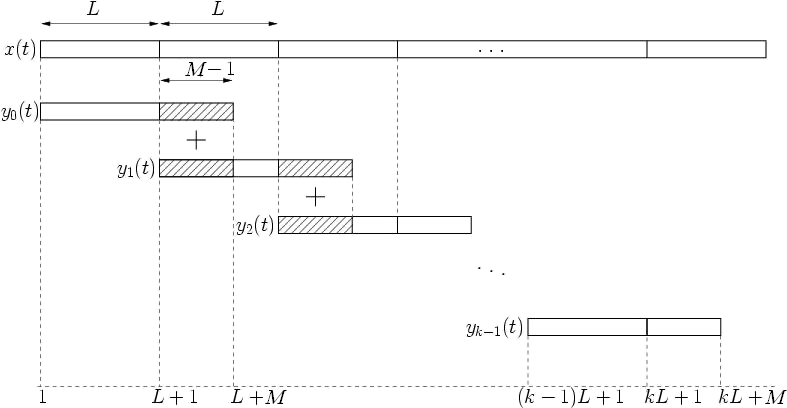
\includegraphics[width=0.8\linewidth]{overlapadd.png}
    \label{fig:overlapadd}
    \caption{Generic Overlap Add (in our case, L=2M, so the overlap ratio is 50\%)}
  \end {figure}

\pagebreak

\subsection{Implementation of the Overlap Add FFT}

To take the Zero padded length $2N$ FFT of a signal of length $N$, we can simply remove the input buffer to the first butterfly, and feed the input stream to
the $n$ of the input butterfly and \emph{0} to the $n+\frac{N}{2}$ input. This puts data through the pipeline faster (as each butterfly will be active every clock, instead of
every other), but the alignment works. Here is an example of using our 8 point FFT to apply an FIR filter of up to length $5$ in the time domain.
Slightly more muxing logic is needed to accomadate the fact that now each butterfly will process data each clock, but the ideas  are the same.
The user would have programmed the (8) Coefficients in the frequency domain in bitreverse order into Coefficient Ram. We would have seperated them
into two rams, 0 $\rightarrow$ N/2-1 and N/2 $\rightarrow$ N-1

      In this case, each forward stage \emph{m} needs input storage of $N/2^{m}$ and ouput storage of $N/2^{m+1}$ (expect for the first butterfly).

  \begin{figure}[h!]
    \centering
    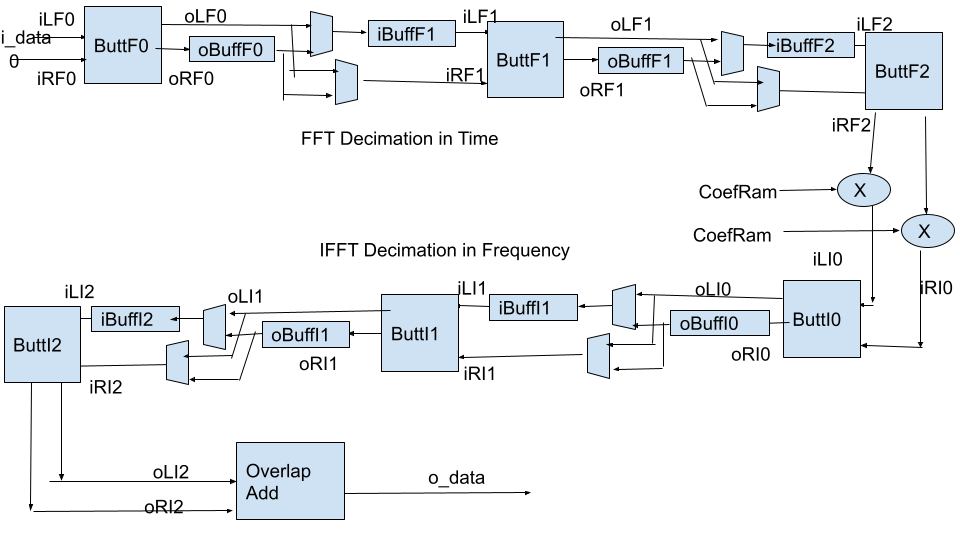
\includegraphics[width=0.7\linewidth]{fft_fir.png}
    \label{fig:fir}
    \caption{4-point Pipelined Overlap Add FIR}
  \end {figure}


Overall the muxing is more complex, and data is processed every clock, but less memory is needed.
The same edits can be applied to the Ifft.

\pagebreak

\subsubsection{Implemenatation of the Overlap and Add Rams}

  \begin{figure}[h!]
    \centering
    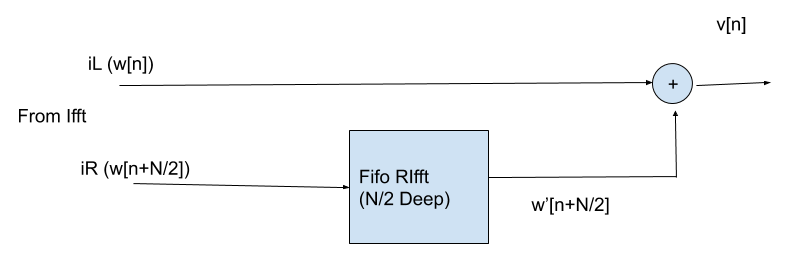
\includegraphics[width=0.8\linewidth]{overlapadd_rams.png}
    \label{fig:overlap_add_rams}
    \caption{Implementation of Overlap Add}
  \end {figure}


We need to combine the results of 2 FFTs, Ie $y_{A}[N/2-1]$ with $y_{B}[0]$, $y_{A}[N/2]$ with $y_{B}[1]$, etc.
In addition, the IFFT will always output 2 samples at a time $y[i]$ and $y[i+N/2]$. (I will refer to these as left(L) and right(R))
The idea will be, for subsquential FFTs A,B,C, ...; We need to combine $A_{R}$ with $B_{L}$, and $B_{R}$ with $C_{L}$, etc.

Each clock, we store the incoming Right sample into the fifo, and output the left signal added with the right signal popped from the fifo.

We are now done!

\end{document}
